\recipe{Ceri's Pad Thai}
\label{recipe:pad_thai}
\makes{2 portions}
\worktime{\SI{10} \minute}
\totaltime{\SI{10} \minute}
\source{\href{https://www.bbcgoodfood.com/}{short link to source}}


\begin{ingredients}

  \item \SI{114}{\gram} rice noodles
  \item \SI{227}{\gram}chicken, tofu or prawns
  \item salt and pepper to taste
  \item 1 large shallot, finely diced
  \item 4 fat garlic cloves, roughly chopped
  \item 2 eggs, whisked
  \item 1 lime
  \item \SI{156}{\gram} bean sprouts
  \item For the sauce:
  \item \SI{3}{\tablespoon} fish sauce
  \item \SI{3}{\tablespoon} brown sugar
  \item \SI{3}{\tablespoon} of rice wine vinegar
  \item \SI{2}{\teaspoon} soy sauce
\end{ingredients}


\begin{method}
  	Place noodles in a pan and cover with boiling water for 4-7 minutes, stirring occasionally until al dente;
drain, rinse with cold water to stop cooking. 

	Whisk the two eggs in a bowl with a a generous pinch of salt. Set aside.
	
	Whisk fish sauce,  rice vinegar, brown sugar and soy sauce in a small bowl and set aside.
	
	Prep the protein. Chicken: slice chicken into very thin strips and add salt and pepper. Crispy Tofu: Dry
tofu with paper towels pressing down firmly. Cut into cubes, sprinkle with salt and pepper, and for extra
crispy, add a little corn starch. Prawns: season with salt and pepper.

	Heat oil in a large saucepan/wok, over medium-high heat. Sear the protien until cooked through, then
set aside. 

	Heat a little more oil in the wok over medium heat, add shallot \& garlic and stir fry 2-3 minutes.  Scoot
the shallot mixture to the side of the pan, add more oil, and pour in the eggs. Scramble and break them
apart into little bits, and move them to the side. Add more oil, and the noodles, stirfry 2-3 minutes until
noodles are soft and pliable and even a little crispy. 

	Pour in the Pad Thai Sauce then add the cooked protein and stirfry for a few more minutes. Just as you
start to smell the sugar carmelizing. Take off the heat and squeeze with a little lime juice. 

	Toss in 1/2 the bean sprouts and roasted peanuts (or serve on the side) and sprinkle with chili flakes and
scallions. Give one more toss and serve :)

  
\end{method}


\begin{figure}[h]
  	\centering
  	
  	\begin{tikzpicture}
  		% Save the image in a box to get its dimensions
  		\sbox0{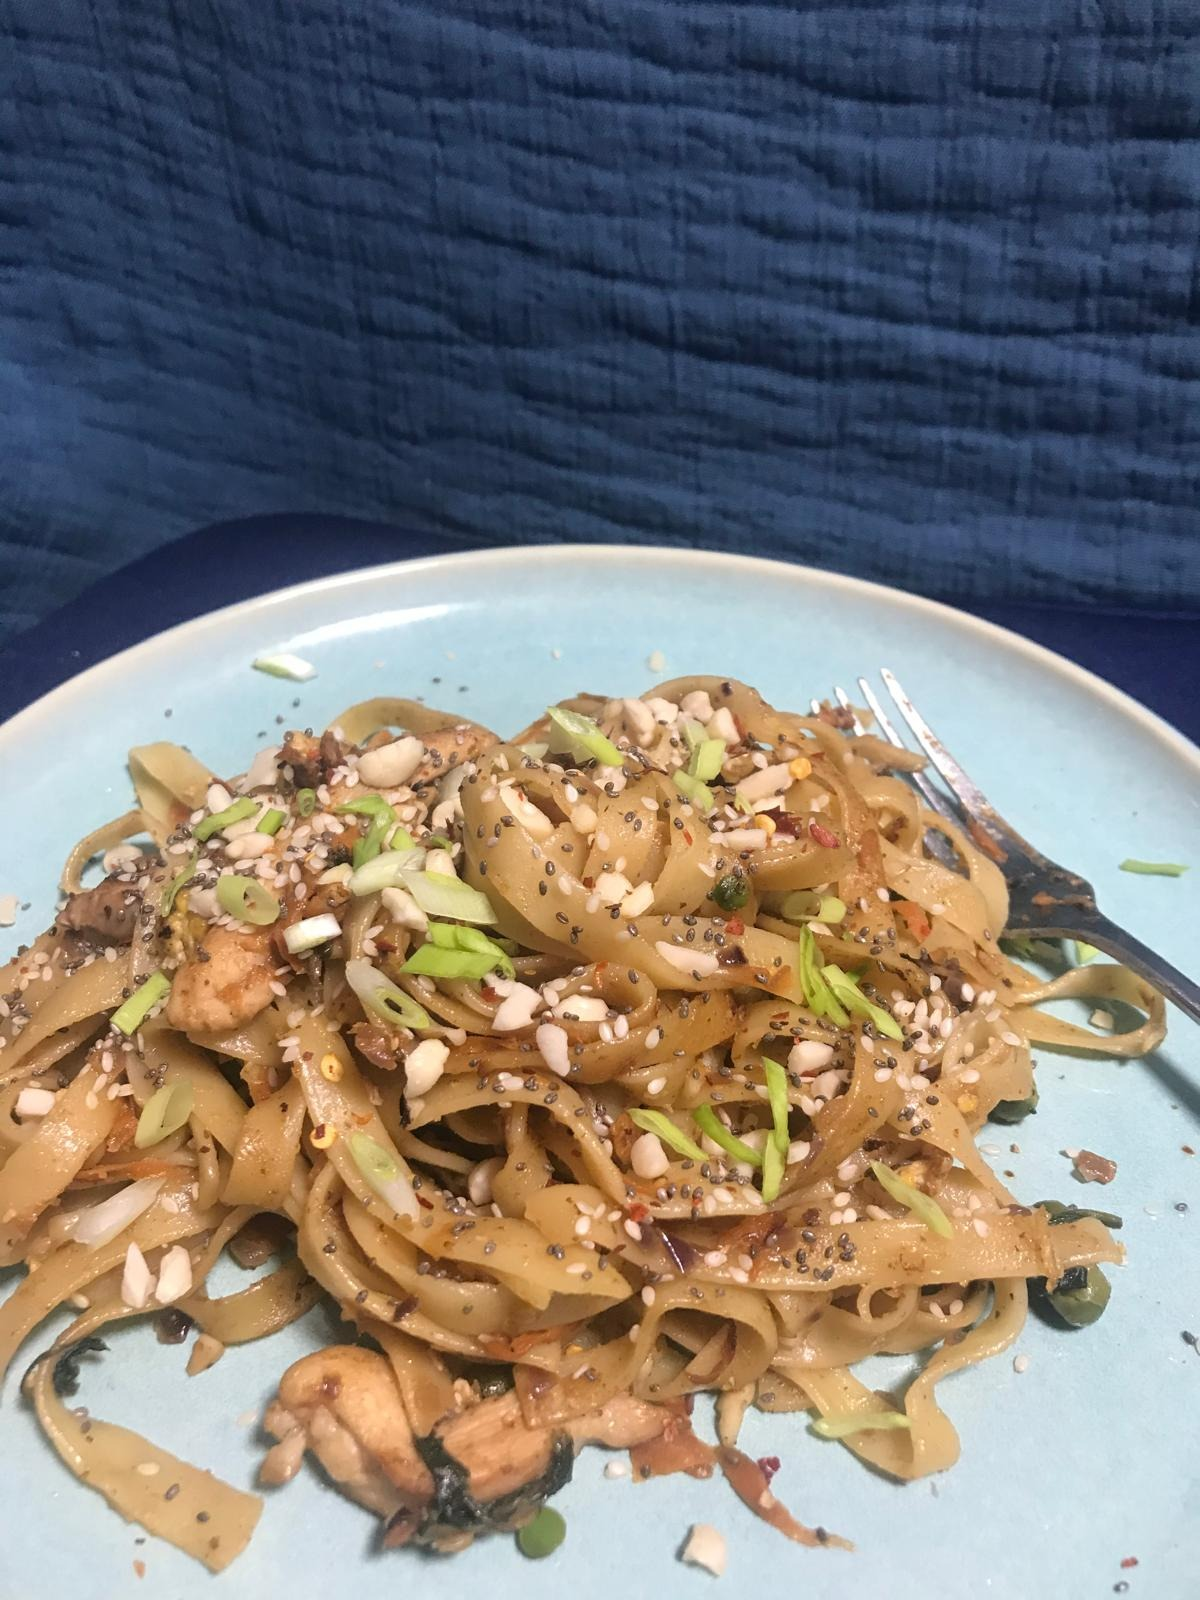
\includegraphics[width = 0.4\linewidth]{images/padThai.jpeg}}%
  
  		% Draw a clipping rectangle with rounded corners
  		\path[clip, rounded corners=0.5cm] (0,0) rectangle (\wd0,3.5cm);
  
  		% Place the image inside the clipped area
  		\node[inner sep=0pt, outer sep=0pt, anchor=south west] at (0,0) {\usebox0};
	\end{tikzpicture}
\end{figure}

